\chapter{Introducción}
%\chapterquote{Hablaban siempre de dinero y planeaban asaltar un banco}{Domingo Cavallo, 2001}

\section{Plantemiento de problema}
\label{S:planteamiento de problema}

\section{Solución propuesta}

Para abordar el problema planteado, el presente Proyecto Final Integrador propone el desarrollo y la validación de un entorno experimental denominado "HW - RT - Reporter".

La solución se centra en el diseño e implementación de un Módulo Reporter en la Lógica Programable (PL) de una placa FPGA, el cual se encargará de monitorear un procesador soft-core (RISC-V) sintetizado en la misma PL. El Módulo Reporter actuará como un bloque de comunicación y de asignación de timestamp confiable por cada evento de interes.

El sistema completo operará bajo una arquitectura que integra el soft-core y el Módulo Reporter, interconectados mediante un bus estándar (protocolo AXI), y comunicándose con un procesador ARM embebido (Processing System - PS) que ejecutará un sistema operativo Linux. El Linux en el ARM servirá como plataforma para recibir, almacenar y procesar los reportes de eventos.

La Hipótesis central de este trabajo es que es posible generar una señal de referencia desde el procesador sintetizado que, al ser observada desde el ARM, permita registrar un timestamp confiable, y que la coincidencia de los timestamps internos con mediciones externas (dentro de un margen de error) validará la precisión del sistema para ofrecer reportes en tiempo real


\subsection*{Objetivos generales}
\label{S:doble-faz}

Diseñar un setup que sea capaz de trackear registros de interes, permitiendo conocer el tiempo que fue abordada una instrucción, para luego poder etiquetarlo y reportarlo con su respectivo \textit{timestamp}.

\subsection{Objetivos puntuales}

\begin{itemize}
\item Adquirir y sistematizar la información técnica necesaria para la correcta selección del \textit{setup} experimental, evaluando distintas opciones de placa, configuraciones de hardware y herramientas de desarrollo.
        
\item Diseñar e implementar un módulo de comunicación entre el \textit{soft-core} y el procesador ARM, garantizando la transferencia de datos en tiempo real y la sincronización de eventos.

\begin{figure}[H]
		\centering
		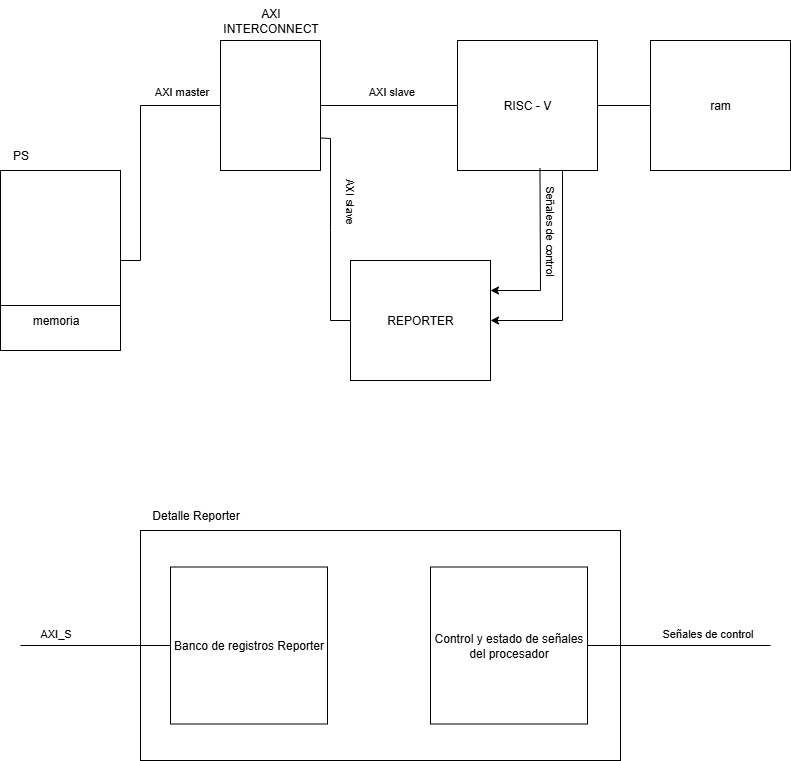
\includegraphics[width=0.65\textwidth]{figs/Diagram_architecture_general.png}
		\caption{Diagrama propuesto para la arquitectura general}
		\label{fig1}
	\end{figure}

\item Evaluar el desempeño del sistema implementado, midiendo métricas como latencia de comunicación, capacidad de respuesta y confiabilidad en la captura de eventos.
\end{itemize}

\section{Estructura del documento}
\label{S:otras-opciones}
Otras opciones con las que se cargue el estilo se pasan directamente a los estilos usados. Por ejemplo si usamos:\\
\verb|\documentclass[11pt,screen,oneside,preprint,draft,pagebackref]{unrnpfi}|\\
producir\'{a} un documento con letra de menor tama\~{n}o (11pt), no se procesar\'{a}n los gr\'{a}ficos (draft) para una mayor velocidad, se producir\'{a}n links en el archivo pdf con la caracter\'{\i}stica adicional que las referencias tendr\'{a}n un link al lugar donde fueron citadas ya que la opci\'{o}n \verb|pagebackref| se pasa al paquete \verb|\hyperref|.

%%% Local Variables: 
%%% mode: latex
%%% TeX-master: "main"
%%% End: 
